\documentclass[times, 09pt, twocolumn]{article}
\usepackage{latex8}

\usepackage[T1]{fontenc}
\usepackage[latin1]{inputenc}

\usepackage{times}
\usepackage{cite}
\usepackage{url}
\usepackage{graphicx}

\begin{document}

\title{Towards an adaptive middleware for opportunistic environment:\\ a mobile agent approach}

\author{Vinicius Pinheiro, Alfredo Goldman\\
Dept. of Computer Science, Universidade de S\~ao Paulo, Brazil\\
\{vinicius,gold\}@ime.usp.br}

\maketitle
\thispagestyle{empty}

\begin{abstract}

The mobile agent paradigm has emerged as a promising alternative to overcome
the construction challenges of opportunistic grid environments.
This paradigm can be used to implement mechanisms that enable the
execution progress of applications even in the presence of failures, such as
the mechanisms presented by the middleware MAG (Mobile Agents for Grid
Computing Environment). 
%MAG explores this powerful paradigm
%by dynamically loading sequential grid applications into mobile agents. These
%MAG agents can be dynamically reallocated to grid nodes through a transparent
%migration mechanism as a way to provide load balancing and support for
%non-dedicated nodes. 
MAG includes retrying, replication and checkpointing as
fault-tolerance techniques. However, they operate independently from
each other and apart from the changes that may happen in the execution environment.
In this paper, we propose adaptive fault-tolerant mechanisms based on dynamic task
replication and checkpointing in order to react to different scenarios of resource
availability.

% don't perform any
% automatic adjustments to adapt themselves regarding those changes.
% Instead, they  
% These mechanisms can be applied in a flexible
% manner, since the user can combine them in order to meet different scenarios of
% resource availability. In this paper we describe the MAG architecture and what
% it can do in a volunteer computing environment. We also propose a
% fault-tolerant mechanism based on dynamic task replication and checkpointing in
% order to meet different scenarios of resource availability. 
\end{abstract}

%============================================================================

\section{Introduction}
% TODO missing references 

Opportunistic grids are distributed environments built to leverage the
computational power of idle resources geographically spread across different
administrative domains. These environments comprise many characteristics such as
high level of heterogeneity and large changes on resource availability. 

%The central element of an opportunistic grid infrastructure is its middleware.
%The grid middleware hides the complexity related to distribution, heterogeneity
%and must efficiently address several issues, such as management and allocation
%of distributed resources, task scheduling, fault tolerance, support for high
%scalability and great diversity of software and hardware components, protection
%and security requirements.
 
%These agents can be used to implement
%mechanisms that enable the progress on the execution of applications even in
%the presence of failures.  These mechanisms can be combined in a flexible
%manner to meet different scenarios of resource availability. In this work, we
%describe the architecture of the MAG middleware (Mobile Agents for grid
%Computing Environment) and what it can do in a opportunistic grid environment.
%We use this middleware as a foundation for the proposal of a adaptive fault
%tolerance mechanism based on task replication and checkpointing. Finally, we
%analyze experimental and
%simulation results.

In distributed systems such as opportunistic grids, failures can occur due to
several factors, most of them related to the resources heterogeneity and
distribution. These failures together with the usage of the resources by its
owners modify the availability status of the resources in the grid (i.e.
resources can be active, busy, offline, crashed, etc) and the middleware should
be able to monitor and detect such changes in order to reschedule the
applications among the available resources or dynamically tune the fault
tolerance mechanisms to obtain a better adequacy to the actual scenario of
availability. 

In this work, we implement dynamic fault tolerance mechanisms for grid
applications. These mechanisms compose a feedback control system
\cite{tanenbaum02}, gathering and analyzing information about the execution
progress and adjusting its behavior accordingly. To build these mechanisms we
rely in the mobile agent paradigm~\cite{pham98}. Mobile agents are programs that can move
from one resource to another in an autonomous way carrying its data and
execution state to resume its execution at the destination. We argue that these
agents exhibits good adequacy for dealing with the complexity related to the
construction of opportunistic grids due to intrinsic characteristics, such as:

\begin{enumerate}
    \item \emph{Cooperation}: agents have the ability to interact and cooperate
    with other agents; this can be explored for the development of complex
    communication mechanisms among grid nodes;
   
    \item \emph{Autonomy}: agents are autonomous entities, meaning that their
    execution goes on without any or with little intervention by the clients
    that started them. This is an adequate model for submission and execution
    of grid applications;
  
    \item \emph{Heterogeneity}: several mobile agent platforms can be executed
    in heterogeneous environments, an important characteristic for better use
    of computational resources among multi-institutional environments;
  
    \item \emph{Reactivity}: agents can react to external events, such as
    variations on resources availability;
  
    \item \emph{Mobility}: mobile agents can migrate from one node to another,
    moving part of the computation being executed and providing load balancing
    among grid nodes.
  
    %\item \emph{Protection and Security}: several agent platforms offer
    %protection and security mechanisms, such as authentication, cryptography
    %and access control.
\end{enumerate}

Since 2004, our research group has being working on applying the agent paradigm
for developing a grid software infrastructure, leading to the MobiGrid and MAG
projects \cite{barbosa04,lopes05}. These projects are based on the middleware
InteGrade \cite{goldchleger04} that follows an opportunistic approach, where
idle computing power of personal workstations is used for executing
computationally-intensive parallel applications.

%Two execution models are supported by the developed infrastructure: regular and
%parametric (or bag-of-tasks) model. The parametric model can be applied to a
%wide range of grid applications. In this case, multiple copies of a single
%binary are executed on different grid nodes. Each process receives a sub-set of
%the application input data and carries out its computation in parallel with the
%others, without requiring any communication among them.
%
%In this scenario, the likelihood of errors is exacerbated due to several
%reasons: each process must successfully finish its execution in order to
%generate a successful application execution; grid applications usually perform
%complex computations, requiring large execution times; opportunistic grid
%environments are very dynamic since the user can request at any time exclusive
%use of resources (workstations).

\subsection{Contributions and Paper Organization}

This work describes improvements to the MAG grid middleware for
efficiently address the high dynamic of the opportunistic
environments, providing an effective management for long sequential and
parametric applications and the allocation of resources necessary for its
successful execution.

% FIXME rewrite this paragraph.
On the next section we present some of the related work. On
Section~\ref{sec:arch} we present the MAG architecture and its fault tolerance
mechanisms. On Section~\ref{sec:adapt} we describe the implementation
of the dynamic replication and the unified checkpointing mechanisms. We provide
some experimental results to evaluate our proposal on Section~\ref{sec:eval}.
Finally, on the last section, we present our conclusions and next goals.


%============================================================================

\section{Related Work}
% Cite UWAgents, CoordAgents e GridWFS (lookup master dissertation)

There are several works that are related to this paper, some related to the
systems giving support for parametric applications, some related to
running long sequential applications on non-dedicated environments, and finally
some works are related to the use of mobile agents on grid middleware.

The most well known work was provided by research on extraterrestrial life on
the SETI program~\cite{seti} where more attention were paid on security aspects
and on the reliability of the results. More recently, the BOINC
project~\cite{boinc} proposed an infrastructure allowing the execution of
different programs which can be executed on volunteer computers spread around
the world. There exist similar projects both with a fixed algorithm as
Mersenne~\cite{mersenne}, and where different algorithms or challenges can be
programmed~\cite{distributed}. However, on these projects the support for long
running sequential applications is mostly restricted to local checkpoints (with
few exception like~ \cite{climate}, or the use of replication to guarantee the
progress of the individual applications). Another bag-of-tasks approach is
based on OurGrid~\cite{cirne06}, however the main focus is on dealing with
the middleware infrastructure and not on the individual sequential
applications.

Several works deals with checkpointing techniques to guarantee the progress of
sequential long running applications. One that is directly related to our
work is~\cite{hwang03}. In this work the authors studied several approaches to
deal with failures on machines. The handling techniques were: retrying, checkpointing,
replication, and replication with checkpointing. They concluded that in grid
environments with high down-time, as it can happen in opportunistic environments,
the replication with checkpointing outperforms the other ones, using as comparison
the lower completion time.

Several works present the use of mobile agents on grid environments, some using
opportunistic contexts~\cite{fukuda03}, but most of them presents characteristics
more related to the middleware, not the
application~\cite{cao02,cao01,loke03,martino04}. Some of the mobile agent work
were done within our project InteGrade~ \cite{goldchleger04}. The first ideas on
using mobile agents on an opportunistic grid appeared in~\cite{barbosa04} where
an architecture based on Aglets~\cite{aglets} is first presented, and then
evaluated with the use of several replicas in~\cite{barbosa05}. More recently a
work based on the mobile agents framework Jade~\cite{jade} was also
presented~\cite{lopes05,lopes06_2}, where there is application instrumentation, to
provide transparent checkpointing and some work on fault tolerance.

To the best of our knowledge this paper is the first one that
specifically uses mobile agents combined with techniques of
replication and checkpointing, within a grid middleware, to provide
dynamic fault tolerance mechanisms for sequential and parametric applications
on opportunistic environments.

%===========================================================================e

\section{The middleware InteGrade/MAG}\label{sec:arch}
% TODO include architecture description
% TODO write about JADE
% TODO write about fault-tolerance
% TODO include code examples(optional) and screenshots
% TODO cite CORBA

The InteGrade project evolves the development of a grid middleware that
leverages the idle computational power of desktop machines. This project is
maintained by the Institute of Mathematics and Statistics of the University of
S\~{a}o Paulo along with others institutions. 
%InteGrade is based on
%CORBA~\cite{vinoski97}, an industry standard for distributed object systems. InteGrade
%naming service uses CORBA IDL (Interface Definition Language) being accessible
%from a large variety of programming languages and operating systems. 
The InteGrade architecture follows an hierarchy in which each node can assume
different responsibilities. The Cluster Manager is represented by one or more
nodes that are responsible for managing that cluster and performing
communication with other clusters. A Resource Provider node is the one that
exports part of its resources, making them available to grid users. A User Node
is one belonging to a grid user who submits grid applications. As we can see in
figure \ref{fig:integrade}, InteGrade architecture follows a two-tier
intra-cluster hierarchy, and a peer-to-peer based inter-cluster network.

\begin{figure}[th]
\centering 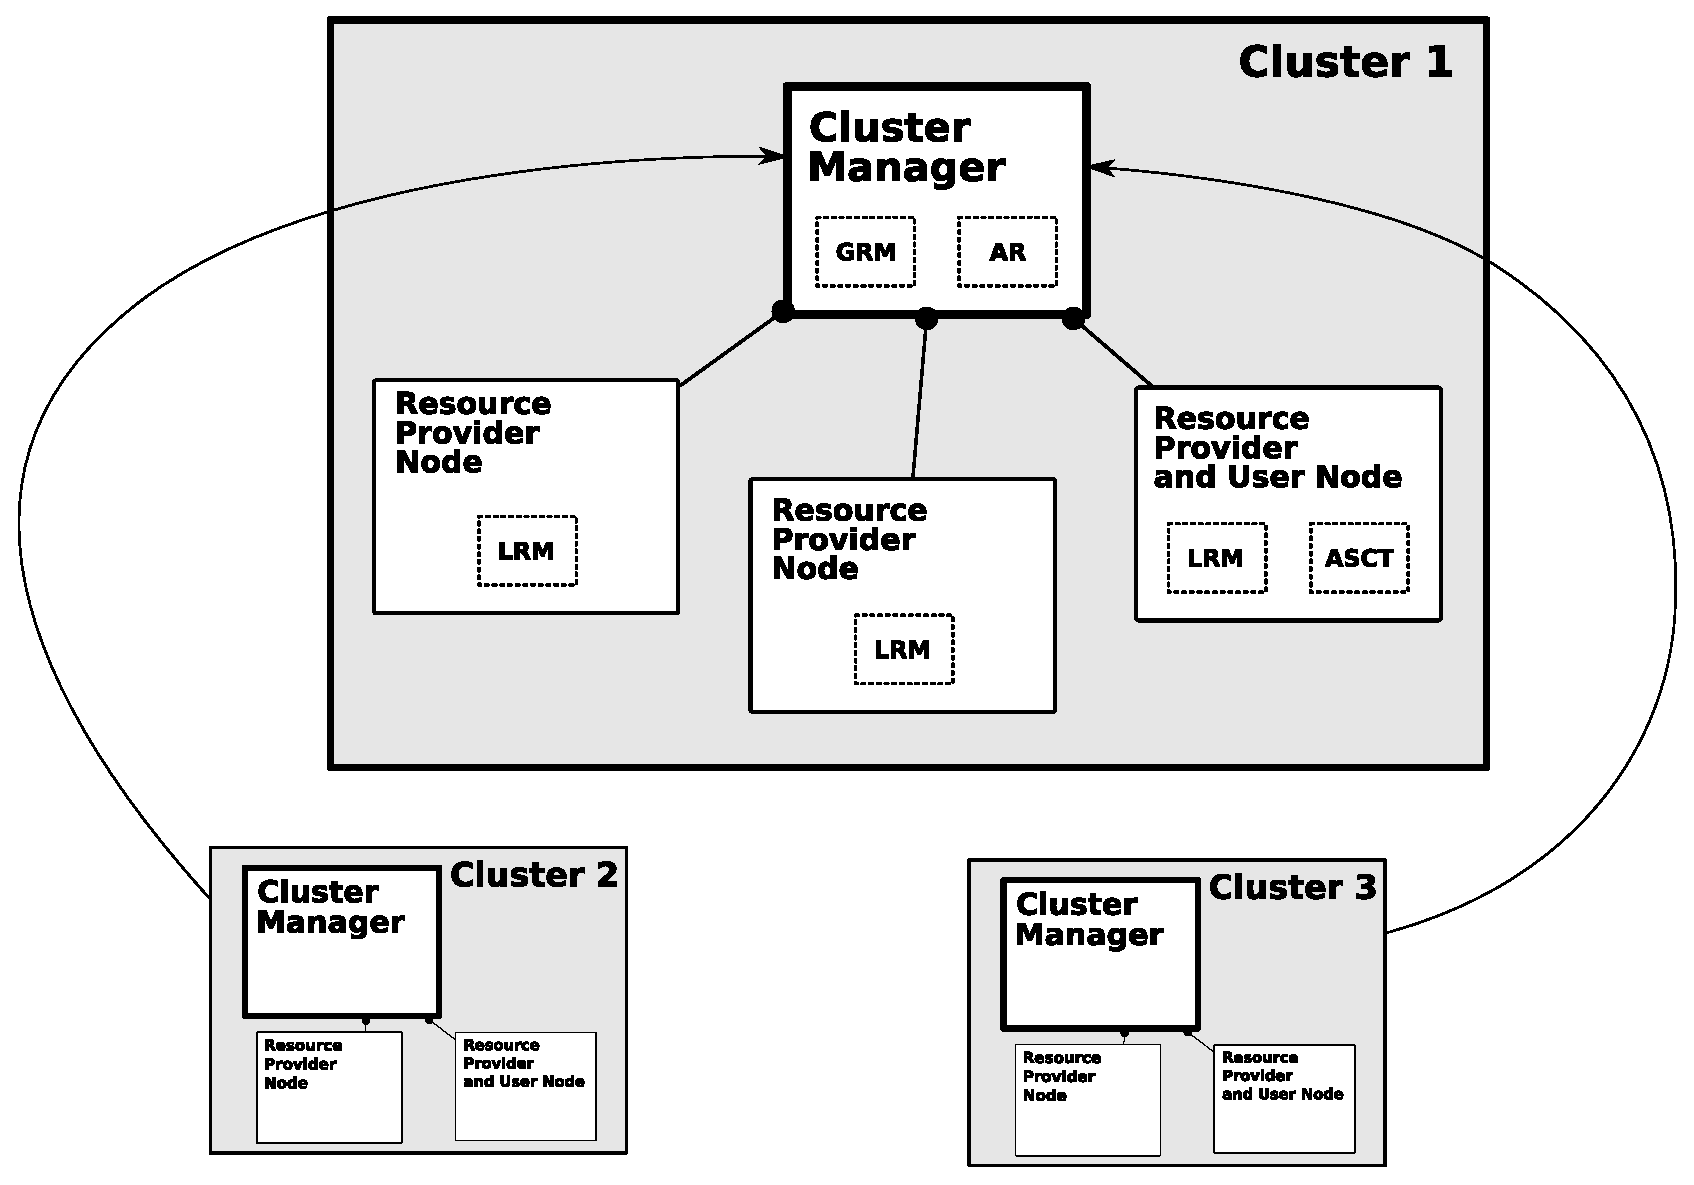
\includegraphics[width=1\columnwidth]{images/integrade2_ieee.eps}
\caption{InteGrade architecture}
\label{fig:integrade}
\end{figure}

The MAG project was developed by the Dept. of Computer Science of the Federal
University of Maranh\~{a}o and introduces the mobile agent technology as new way
of executing applications on InteGrade. Through MAG, the grid user can submit
Java applications, not supported by the native InteGrade middleware. This is
performed by dynamically loading sequential grid applications into mobile
agents. MAG uses JADE (\emph{Java Agent Development Framework}) as the agent
platform to provide agent services such as communication and life cycle
monitoring. 
%Figure \ref{fig:magarch} depicts the architecture layers of the MAG middleware.
%The JADE~\cite{jade} (\emph{Java Agent Development Framework}) layer represents the agent
%platform used by MAG to provide agent services such as communication and life
%cycle monitoring. 
%Jade provides a private queue of messages to each agent
%allowing them to exchange messages specifying their topics and their receivers.
%JADE is portable, since it was implemented in Java, and complies with the
%FIPA~\cite{fipa} specification (Foundation for Intelligent Physical Agents).
%\begin{figure}[th]
%\centering \includegraphics[width=0.7\columnwidth]{images/magarch_en.eps}
%\caption{InteGrade/MAG middleware layers}
%\label{fig:magarch}
%\end{figure}
In order to avoid duplication of efforts, the MAG project was build on top of
some InteGrade components: Global Resource Manager (GRM), Local Resource
Manager (LRM), Application Repository (AR) and Application Submission and
Control Tool (ASCT). The GRM is the main component in the grid and is executed
in the Cluster Manager Node. The GRM holds informations about the registered
LRMs and is able to dispatch tasks to them. The LRM is executed in
each Resource Provider node. It loads the execution environment in order to
execute tasks submitted to them. The AR provides a centralized repository to
store the application binaries. Finally, the ASCT provides a interface in which
the user can submit applications to the grid. The user can also monitor the
execution status and view the results of the execution.

%\begin{enumerate}
%
%    \item \emph{Local Resource Manager (LRM)}: This component is executed in
%each Resource Provider node, loading the execution environment and wrapping the
%application processes delegated to it. LRM also contains a sub-component called
%LUPA (Local User Pattern Analyzer) that collects informations about memory and
%CPU utilization. The LRM sends status information about applications in
%execution. It also sends heartbeat messages periodically.
%
%    \item \emph{Global Resource Manager (GRM)}: This is the main component in
%the grid and is executed in the Cluster Manager Node. The GRM holds
%informations about the registered LRMs and is able to send tasks to them.
%
%    \item \emph{Application Repository (AR)}: This component provides a
%centralized repository to store application binaries that will be submitted for
%execution.
%
%    \item \emph{Application Submission and Control Tool (ASCT)}: This component
%is executed in the User Node and provides a interface in which the user can
%submit applications to the grid. The user can also monitoring the execution
%status and view the results of the execution.
%
%\end{enumerate}

Besides those, MAG architecture adds some others components that provides
mobile agents capabilities and fault-tolerance mechanisms:

\begin{enumerate}

    \item \emph{ExecutionManagementAgent (EMA)}: This component stores
    informations about current and past executions, as the current execution state
    (accepted, running, finished), input arguments and scheduled machines. This informations
    could be retrieved to restore applications to the point that they were before
    the failure;

    \item \emph{AgentHandler}: This component runs on top of the LRMs. The
    AgentHandler works as a proxy to the JADE agent platform, instantiating
    MAGAgents for each requested execution;

    \item \emph{ClusterReplicationManagerAgent (CRM)}: When the GRM receives a
    execution with replicas request it delegates to the CRM. This component
    processes informations for each replica an create an ERM agent to handle the
    request;

    \item \emph{ExecutionReplicationManagerAgent (ERM)}: This component
    contacts the LRMs of the target machines in order to execute the replicas, one
    in each machine;

    \item \emph{StableStorage}: The stable storage receives the compressed
    checkpoints in order to store them in the file system, and retrieve it when
    receives a query request. This agent runs in the Cluster Manager node;

    \item \emph{MAGAgent}: This is the main component of the MAG middleware.
    The MAGAgent wraps the application, instantiate it, and catch the application
    exceptions that may be raised. It also controls the applications life cycle;

    \item \emph{AgentRecover}: This component is created on demand to perform
    the recovery of the execution in the presence of incidental failures.

\end{enumerate}

\subsection{Fault-tolerance in MAG\label{sec:faulttolerance}}

In this section we present the fault-tolerance mechanisms available on MAG.
This mechanisms can be combined to meet different scenarios of resource
availability, resulting in 4 different strategies:

\begin{enumerate}
    \item \emph{Retrying}: Every time the application fails it is automatically submitted again;
   
    \item \emph{Replication}: Various replicas of the application are submitted
for execution at the same time. When one of the replicas finishes, the others
are discarded to avoid overconsumption of resources. In case of failure,
retrying is applied;
   
    \item \emph{Checkpointing}: The application periodically saves its execution
state in a stable storage. In case of application failure, the retrying is
applied, but the execution is resumed from the most recently checkpoint
state;
 
    \item \emph{Checkpointing with Replication}: Each replica periodically saves
its execution state in a stable storage. Retrying and resuming of execution is
also applied for each replica in the presence of failures.

\end{enumerate}

Currently, the MAG middleware supports only the submission of parametric and
serial Java applications. In order to execute them, its necessary to extends
the {\tt MagApplication} class. This is necessary, so the application code can
be wrapped into a mobile agent and submitted to the agent platform. 
%Next, we
%describe what happens in case of application submission with replicas on MAG
%(figure \ref{fig:submission}):
%
%\begin{figure}[th]
%\centering \includegraphics[width=1\columnwidth]{images/mag_submission.eps}
%\caption{Application submission on MAG}
%\label{fig:submission}
%\end{figure}
%
%The user submits the application through the ASCT interface along with
%informations about its execution (1): input arguments, number of replicas, input
%and output files, etc. The application binary is stored in the AR component (2)
%and the execution request is sent to the GRM (3). After the submission, the GRM
%checks it there are sufficient resources (e.g. number of replicas must not
%exceed the number of LRM nodes) (4). If so, the GRM delegates the
%execution to the CRM (5). The CRM generates an unique id for each replica and
%creates an ERM agent to manage the request (6). The ERM proceeds with execution
%by requesting the LRM's of the target machines (7). Then, each LRM delegates the
%execution to the AgentHandler which creates a {\em MAGAgent} for each
%request (8). The {\em MAGAgent} is responsible for downloading the application binary from
%the AR component(9), instantiate the application, and notify the AgentHandler when
%the execution has finished. 

%All the informations about execution (e.g.  execution time, number of replicas,
%machines used, etc) are placed onto a relational database by the EMA, and can
%be queried later. The {\em GRM} select the {\em LRM}'s to execute the tasks
%performing a round-robin strategy.
%
%In a opportunistic environment many problems can arise during the application
%execution process, e.g. machines being turned off, out of memory errors,
%heisenbugs, etc. This is even more tricky when executing long running
%applications, since they are exposed to these problems during a long period of
%time. When such a failure occurs in the executing environment, the {\tt MAGAgent}
%class overrides an \emph{uncaughtException} method to handle it. This method
%instantiate a local Agent Recover that gather information from the GRM in order
%to get a reference to an AgentHandler of an available node. Finally, the
%Agent Recover requests the remote AgentHandler to restore the execution. It is
%worthwhile to say that this retrying mechanism is provided also to every
%replica, in case of execution with replicas.

In the MAG middleware the checkpoint mechanism is obtained through code
instrumentation provided by the \emph{MAG/Brakes} framework. This
framework is a modified version of the Brakes framework~\cite{brakes00}, developed by the
DistriNet research group, from the Katholieke Universiteit Leuven, Belgium. 
%The
%MAG/Brakes framework performs the capture of the state execution of JAVA
%threads allowing them to resume its executing in another location. The MAG/Brakes also is the
%core of a powerful migration mechanism, since the execution can be interrupted at any time
%and be resumed without loss of computational work. This feature saves efforts from the
%application developers in the sense that there is no need to modified the application
%code to explicit where the checkpoint must be performed. Currently, the MAG/Brakes
%only performs code instrumentation of JAVA applications compiled with previous
%versions of the Java language (1.4 or lower).
%When an instrumented application is executing in MAG, it periodically invokes
%the \emph{setCompressedCheckpoint} method of the {\tt MAGAgent} class. Through this method
%the agent interacts with the {\em StableStorage} component. This component is in
%charge of getting all the compressed execution state and stored it in a local
%file. When the application execution needs to be restored (e.g. a failure happens), the
%\emph{getCompressedCheckpoint} method is invoked to restore the application
%execution state. After that, the application execution is resumed.

\section{Improving MAG: towards an adaptive middleware}\label{sec:adapt}
% TODO use previous results from Francisco and some new experiments with MTBF,
% replication and checkpoint
% TODO write about experiments to simulate the behavior of this adjustment faced to variation on the arrival time between submissions
% TODO describe how to analyze the results

As shown in section \ref{sec:faulttolerance}, the MAG middleware supports
multiple fault-tolerance techniques, but these techniques operate solely.
Besides, they do not perform any automatic adjustments to adapt themselves
regarding changes in the resource availability. If a machine is turned off, for
example, all the replicas that were executing in it are lost as MAG only
detects failures at the application layer. These replicas are not replaced and
the middleware does not make use of theirs respective checkpoints.

%The fault-tolerance mechanisms provided by the MAG middleware 

Events such as network partitioning, crash failures, shutdown of machines,
nodes joining the grid, nodes leaving the grid, etc, define the resource
availability of the executing environment and this may change according to the
frequency of those events. Hence, we propose that MAG should automatically and
dynamically tune its fault-tolerance mechanisms to fit to those changes.

%One can argue that a system administrator may observe the changes that happen
%with the resources at the execution environment and alter the behavior of
%these mechanisms by modifying its execution parameters accordingly, through a
%customized interface. But this is a very complex task since it
%requires very specialized knowledge and full time observation from the
%administrators. Furthermore, it is worthwhile to mention that, in the current
%version of MAG, updating the mechanisms requires the restart of the middleware
%components deployed in the grid.

\subsection{Unified Checkpoint}

As explained previously, the fault-tolerance mechanisms of MAG work
independently from each other. This model have scalability issues since it
implies that all replicas submitted for execution performs checkpointing
periodically, increasing the communication traffic between provider nodes and
the repository and consuming more resources from the grid such as processing
and storage. Another disadvantage of this model is related to the resource
heterogeneity: in a heterogeneous environment like computational grids some
replicas may advance its execution more quickly than others. If the most
advanced replica crashes in a way that MAG cannot detect, its latest checkpoint
will not be used for the late replicas and part of the execution will be
lost. This lost will only be recovered when one of the late replicas achieve
the same point where the crashed replica stopped. 

In response to this problem we propose a mechanism named Unified Checkpoint. In
this new model the replicas periodically send informations about their
execution progress and only the most advanced replica is authorized to perform
checkpointing. To enable this feature the applications must invoke a method
which increases a counter. It is in charge of the application programmer to
choose the most appropriately places to put these invocations into the code
since this is a very application specific issue. When the replica hits a
checkpoint, it sends only the value of the counter and the Stable Storage
compares this value with the ones sent by the other replicas. Only the
replica with the highest counter value will be feedbacked to perform the
checkpointing. This model is exemplified in the figure \ref{fig:repCheckNovo}.

\begin{figure}[th]
\centering 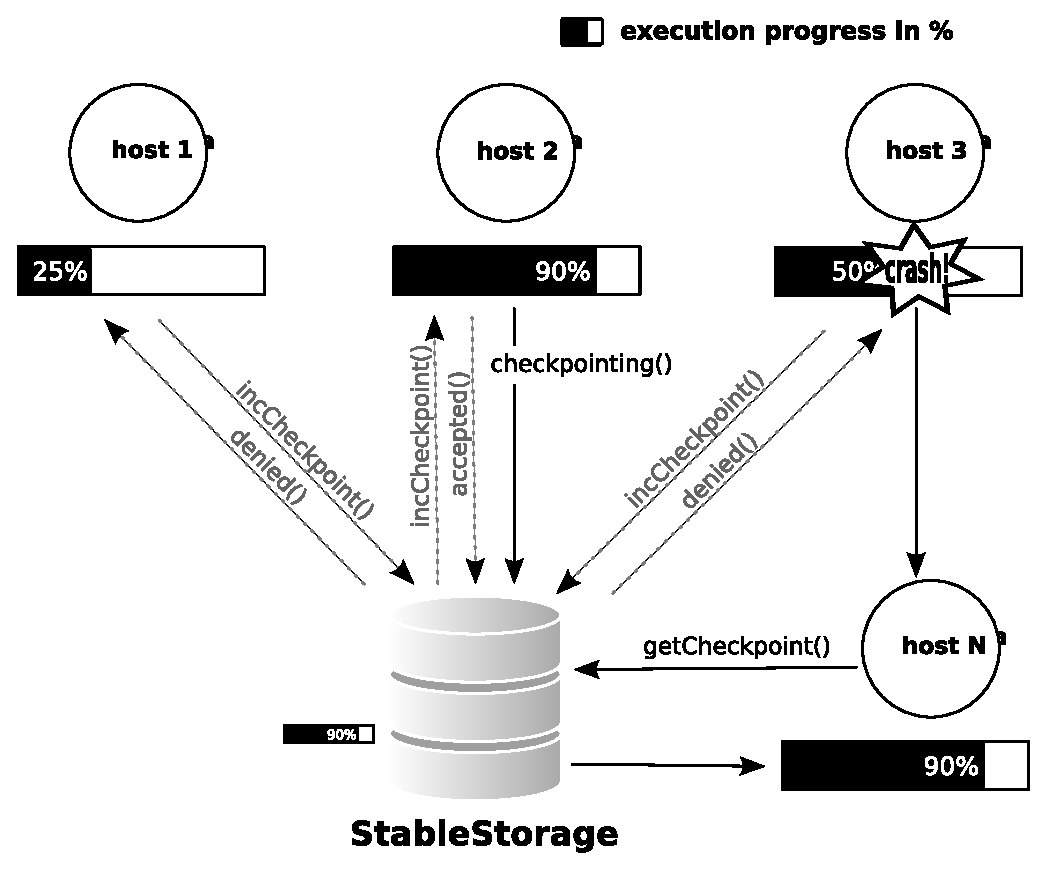
\includegraphics[width=0.9\columnwidth]{repCheckNovoFalha.eps}
\caption{Unified Checkpoint model}
\label{fig:repCheckNovo}
\end{figure}

In this figure the replica running at host 2 is the most advanced one. When
the replica running at host 3 crashes the MAG recovery mechanism took place
and a new replica is created at host N and the Stable Storage is asked for a
checkpoint file. The checkpoint stored by the most advanced replica is the only
option and so this one is sent to the new replica which resumes its execution
from this advanced stage. 

\subsection{Replica Replacement}

Although the checkpointing and the replication of tasks now operate together to
form a more integrated fault tolerance system, some events, like shutdown of
machines for example, may reduce the number of replicas in execution. Besides,
it would be interesting to compare the counters between replicas in order to
detect replicas that are late regarding the distance from the most advanced
replica and decide where it must be substituted for a fresh one, whose
execution will be resumed from the unified checkpoint on another resource.

To fulfill this gap we propose a feedback control system based on periodical
analysis of resource availability. This system is represented in figure
\ref{fig:feedback}.

 
%\subsection{Dynamic replication} 
%
%Although the checkpointing and the replication of tasks now operate together to
%form a more integrated fault tolerance system, these mechanisms are still not
%able to adapt their selfs according to environment changes. To fulfill this gap
%we propose a feedback control system based on periodical analysis of resource
%availability. This system is represented in figure \ref{fig:feedback}.
%
\begin{figure}[th]
\centering 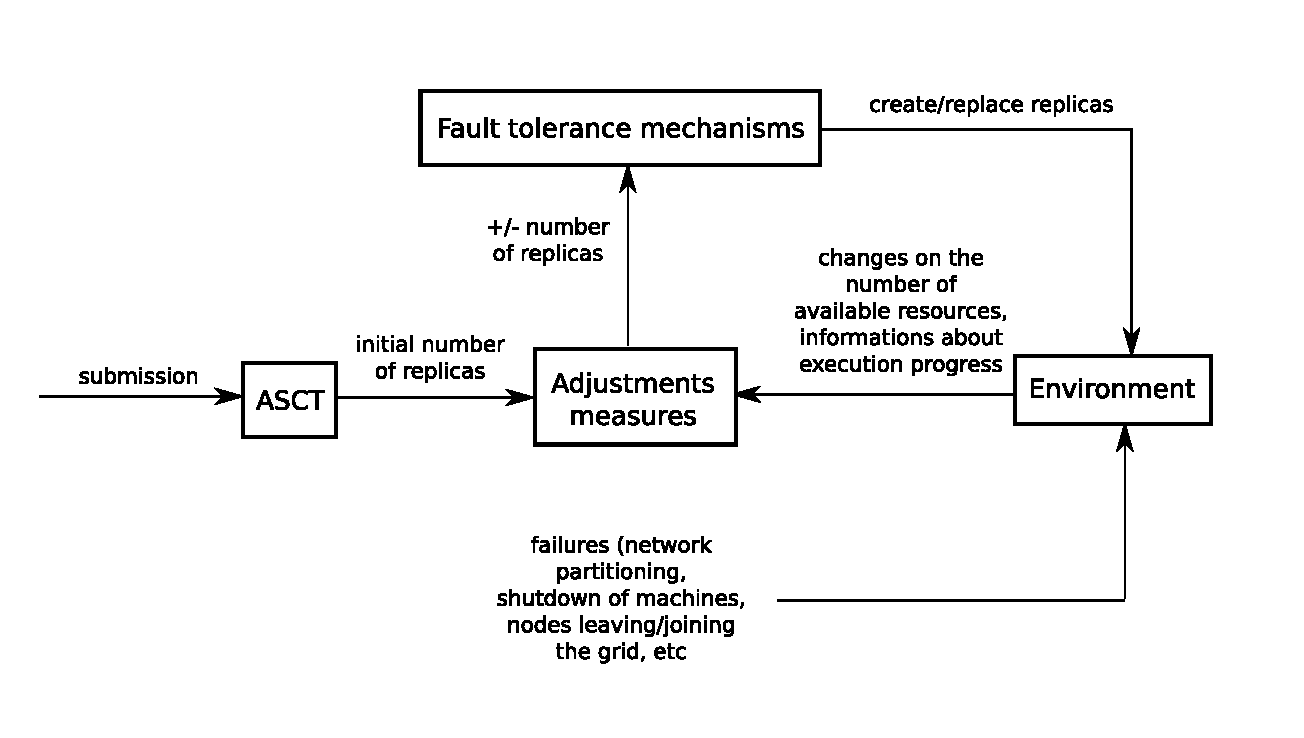
\includegraphics[width=1.1\columnwidth]{feedback.eps}
\caption{Dynamic replication: a feedback system model}
\label{fig:feedback}
\end{figure}
%
Initially, the grid user submit an application in the grid. The application
replicas are created and submitted for execution in the nodes. The number of
replicas created will be equal to fixed number defined by the user, but
respecting a maximum value of replicas for each application \footnote{The
maximum number of replicas allowed can be customized by the grid
administrators}. While running, these replicas are susceptible to failures
related to intrinsic characteristics of opportunistic environments such as
network partitioning, shutdown of machines, out-of-memory errors, etc. These
failures reduce the number of replicas in execution and also modify the number
of available resources. These changes are detected by the system that after a
period without getting response from the crashed/offline nodes, updates the
list of LRM's that are still alive (and the new ones that have joined or
rejoined the grid in this time frame). Furthermore, during this time, some
replicas may become delayed. Based on these informations, new replicas are
created and late ones are replaced and submitted to the fresh available
resources. It is worthwhile to remember that the Unified Checkpoint will be
always present through this process, so new replicas will resume its execution
from the checkpoint of the most advanced replica. This mechanism works even
when the most advanced replica crashes, as its last checkpoint remains stored
at the Stable Storage so that the new replica can resume from it.

%
%If there is more than one application submitted, the number of available
%resources should be uniformly distributed among them. So, when a new
%application is submitted the resources must be redistributed among the
%executing applications and the new application. This is performed by deleting
%some replicas of the executing applications and adding new replicas of the new
%application in a way that all the applications should have the same number of
%replicas. On the other hand, when applications finish its execution this event
%also triggers the adjustments measures in order to add new replicas of the
%applications remaining. 

\section{Experiments and simulations}\label{sec:eval}

In this section, we present an event based simulation in diverse scenarios
demonstrating the potential value of adding dynamic fault-tolerance mechanisms
into MAG. Our analysis will be focused on the execution times of the tasks and
the amount of resources used to execute them. Following are the parameters used
for our simulation (mostly borrowed from \cite{plank98, beguelin97}).

\begin{itemize}
    \item \emph{Failure rate ($\lambda$)}: This is a random variable
representing an arrival rate of failures governed by a Poisson distribution.
TBF (time between two adjacent failures) is a random variable governed by a
exponential distribution with MTBF representing the average;
    
    \item \emph{Downtime (D)}: This is the average time following a failure of a
task before it is up again, governed by the exponential distribution;
   
    \item \emph{Number of replicas (N)}: This is the number of copies of an
application, with each running on different machines.  \end{itemize}

The processing power of the resources where generated randomly from 800 to 1600
based on SPECfp benchmark (Standard Performance Evaluation Corporation). 

We measured the expected time of tasks to compare the performance of the
proposed techniques against the old model. We used 2, 4, 8 and 16 replicas and
fixed 1 hour as the MTBF value to obtain a $\lambda$ of 24 failures per day.
The average downtime was fixed to 30 minutes (1/2 hour). These values were used to
simulate a very inhospitable environment to distributed processing like
student laboratories, where machines are regularly turned off and rebooted.
For each number of replicas we performed 40 simulations and measured the
arithmetic mean and the 95\% confidence interval\footnote{We used the t-Student
distribution} of the execution times. We assumed the application execution time
as the execution time of the replica that finished first. The results are
plotted in figure \ref{fig:adapt-mag}.

\begin{figure}[th]
\centering 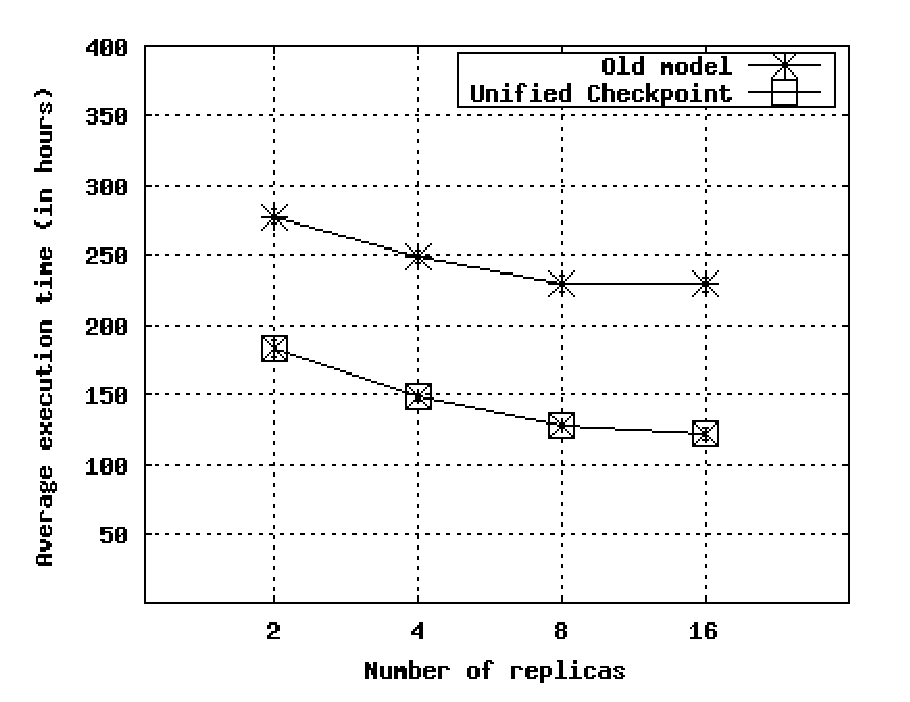
\includegraphics[width=1.1\columnwidth]{49-55_scenario.eps}
\caption{Performance comparison: Unified Checkpoint versus Old model}
\label{fig:adapt-mag}
\end{figure}


First of all, it becomes clear that increasing the number of replicas results
in shorter execution times in both strategies. But we can realize a
considerable gain in the total execution time when using the dynamic strategy
presented in this paper. The potential advantage of adopting the
Unified Checkpoint mechanism occurs independently of the number of replicas used in our
simulation. In all the cases the Unified Checkpoint outperforms the old model
obtaining better execution times (at least 34\% lower). This difference
increases to the extent that the number of replicas increases, achieving its
maximum delta when 16 replicas were submitted (execution time 47\% lower). More
important to say, is that the amount of time saved when using the Unified
Checkpoint varies between 95 and 107 hours. 
%
%For evaluation purpose, we use a dummy application that call repeatedly a
%method for string concatenation. Despite its simplicity, this is a worst case
%application for our checkpoint experiments, since the code instrumentation of
%MAG/Brakes framework happens in the applications methods calls.
%
%Following are the parameters we used in our evaluation:
%
%\begin{enumerate}
%    %\item \emph{Failure-free execution time (FF)}: This is the amount of time to
%    % execute the application in absence of failures.
%   
%    \item \emph{Mean-time between failures (MTBF)}: This is the average time a
%failure occurs in the execution environment.
% 
%    \item \emph{Number of Replicas}: This is the number of replicated
%tasks.   
%\end{enumerate}
%
%We used 0, 1, 3 and 5 number of replicas in our evaluation, and for each number
%of replicas we fixed 0,5 (30 seconds) as the MTBF value. This can be considered
%a severe MTBF value considering the simulations results in \cite{sallem07}. We
%chose this value to effectively measure the efficacy of the fault-tolerance
%mechanisms. The ERM component was modified to generate the failures according to
%a provided MTBF value. The ERM periodically invokes a random function that
%returns \emph{true} or \emph{false}. If \emph{true} the failure is generated
%and the node collapses, otherwise nothing happens. This function is invoked
%each 10 seconds so that every time it is invoked the probability or returning
%\emph{true} is 1/3 (for MTBF = 0,5). Due to time restrictions, we simulate 24
%minutes as 24 hours in our evaluation. Doing so, we could do more executions in
%a short time period to obtained results within a acceptable statistical
%relevance.
%
%
%%TODO replication (without checkpoint) is essential to our propose, but I think we do not have
%% to much time for it.
%
% 
%\subsection{Expected Results}
%
%Based on that values we measured the total execution time of the application
%when using the \emph{Checkpointing with Replication} strategy. 
%For each number of replicas
%we performed 40 simulations and measured the arithmetic mean of the execution
%time. We assumed the application execution time as the execution time of
%the replica that finished first. 
%The results are plotted on
%figure~\ref{fig:repCheck}. i
%We can realize a
%considerable gain in the total execution time when using the dynamic strategy.
%For instance, we can see a clear advantage by using 3 replicas
%instead of 1, and when using 5 replicas the total execution time fails to
%almost the half of the time when executing with no replicas.
%
%
%\begin{figure}[th]
%\centering \includegraphics[width=0.85\columnwidth]{images/graphModel.eps}
%\caption{Checkpoint with replication evaluation}
%\label{fig:repCheck}
%\end{figure}
%

\section{Conclusion}

The grid middleware hides the complexity related to distribution and
heterogeneity and must efficiently address several issues, such as management
and allocation of distributed resources, dynamic task scheduling, fault
tolerance, support for high scalability and great heterogeneity of software and
hardware components, protection and security requirements. 

Mobile agents paradigm exhibits great adequacy for dealing with the complexity
of building the grid software infra-structure due to its intrinsic
characteristics, such as cooperation, autonomy, heterogeneity, reactivity,
mobility among others. In this work, we present the Unified Checkpoint
mechanism, which combines dynamic task replication, replica substitution and
checkpointing to provide fault tolerance for sequential and parametric
applications. We use the MAG middleware as the basis for implementing these
mechanism. This middleware makes benefit from the mobile agent paradigm to
encapsulate the applications submitted to the grid. 

We demonstrated through our experiments that, in opportunistic environments,
it is crucial to support dynamic fault tolerance mechanisms in order to
achieve high performance as well as to make a better use of the available
resources even in a highly heterogeneous and instable environment.

Currently, we are investigating other self-optimization and adaptive mechanisms
to introduce in our feedback system. We are measuring the benefits of increasing
or decreasing the number of replicas accordingly to three factors: failure rate
of the execution environment, number of free resources and amount of tasks to
be scheduled. We are also investigating the impact of changing the
checkpointing interval accordingly to the failure rate and the size of the
checkpoints, in order to optimize the completion time of the applications. 

%============================================================================
\bibliographystyle{latex8}
\bibliography{bibliografia}

\end{document}
